\chapter{Monte Carlo simulation corrections}\label{chap:MCCor}
\minitoc

Monte Carlo simulation plays an important role in the cross section measurement, therefore should have a best possible agreement with the data. Part of these corrections are described in Chap.~\ref{chap:MC}. Some of the discrepancies between data and MC simulation are corrected using the reconstructed events. There are two possible methods to correct MC simulation: application of the weights on MC events (reweighing) and random changing of reconstructed 4-vectors (smearing).

This chapter describes all additional corrections, that are applied to MC simulation samples in this analysis.

\section{Lepton efficiency corrections}\label{sec:Eff}

The efficiency of the lepton selection at the \atlas detector can be divided into three components:
\begin{itemize}
\item The reconstruction efficiency $\epsilon_{rec}$. It is a probability to reconstruct lepton as a lepton of this flavor;
\item The identification efficiency $\epsilon_{id \mid rec}$. It is a probability that a reconstructed lepton survives  identification requirements;
\item The trigger efficiency $\epsilon_{trig \mid rec,id}$. It is a probability, that the lepton satisfies the trigger requirements. 
\end{itemize}

The full selection efficiency for a single lepton can be written as:
\begin{equation}
\epsilon_{total}=\epsilon_{rec} \times \epsilon_{id \mid rec} \times \epsilon_{trig \mid rec,id}.
\end{equation}

The efficiencies are measured using the tag-and-probe method with $Z\to ll$ decays.  One of the leptons from the Z-boson, called "tag", is initially selected with the stricter set of selection. Second, "probe" electron candidate, is used for the efficiency measurements.

The single lepton efficiencies can be translated to the corresponding efficiency for the detection of a lepton in W and Z-boson decays :
\begin{equation}
\epsilon^{W}_{total}=\epsilon_{rec} \times \epsilon_{id \mid rec} \times \epsilon_{trig \mid rec,id},
\end{equation}
\begin{equation}
\epsilon^{Z}_{total}=\epsilon_{rec} \times \epsilon_{id \mid rec} \times (1+(1-\epsilon_{trig \mid rec,id})^2).
\end{equation}

Reconstruction efficiency is associated with the algorithm used in the event reconstruction process. In the electron channels, the reconstruction efficiency is defined as a probability to reconstruct electron given the presence of the cluster.  

The muon reconstruction efficiency is estimated as:
\begin{equation}
\epsilon_{reco,muon} = \epsilon_{reco,muon|ID} \cdot \epsilon_{ID} \approx \epsilon_{reco,muon|ID} \cdot \epsilon_{ID|MS},
\end{equation}
where $\epsilon_{reco,muon|ID}$ is the probability to reconstructed in ID is also reconstructed using MS as a combined muon, and  $\epsilon_{ID}$ is an efficiency of muon reconstruction given the ID track. The identification efficiency $\epsilon_{ID}$ cannot be measured directly  in the data and therefore can be approximated by the value of $\epsilon_{ID|MS}$ efficiency to reconstruct muon in MS given the ID track. 



\begin{figure}[!tbp]
\centering
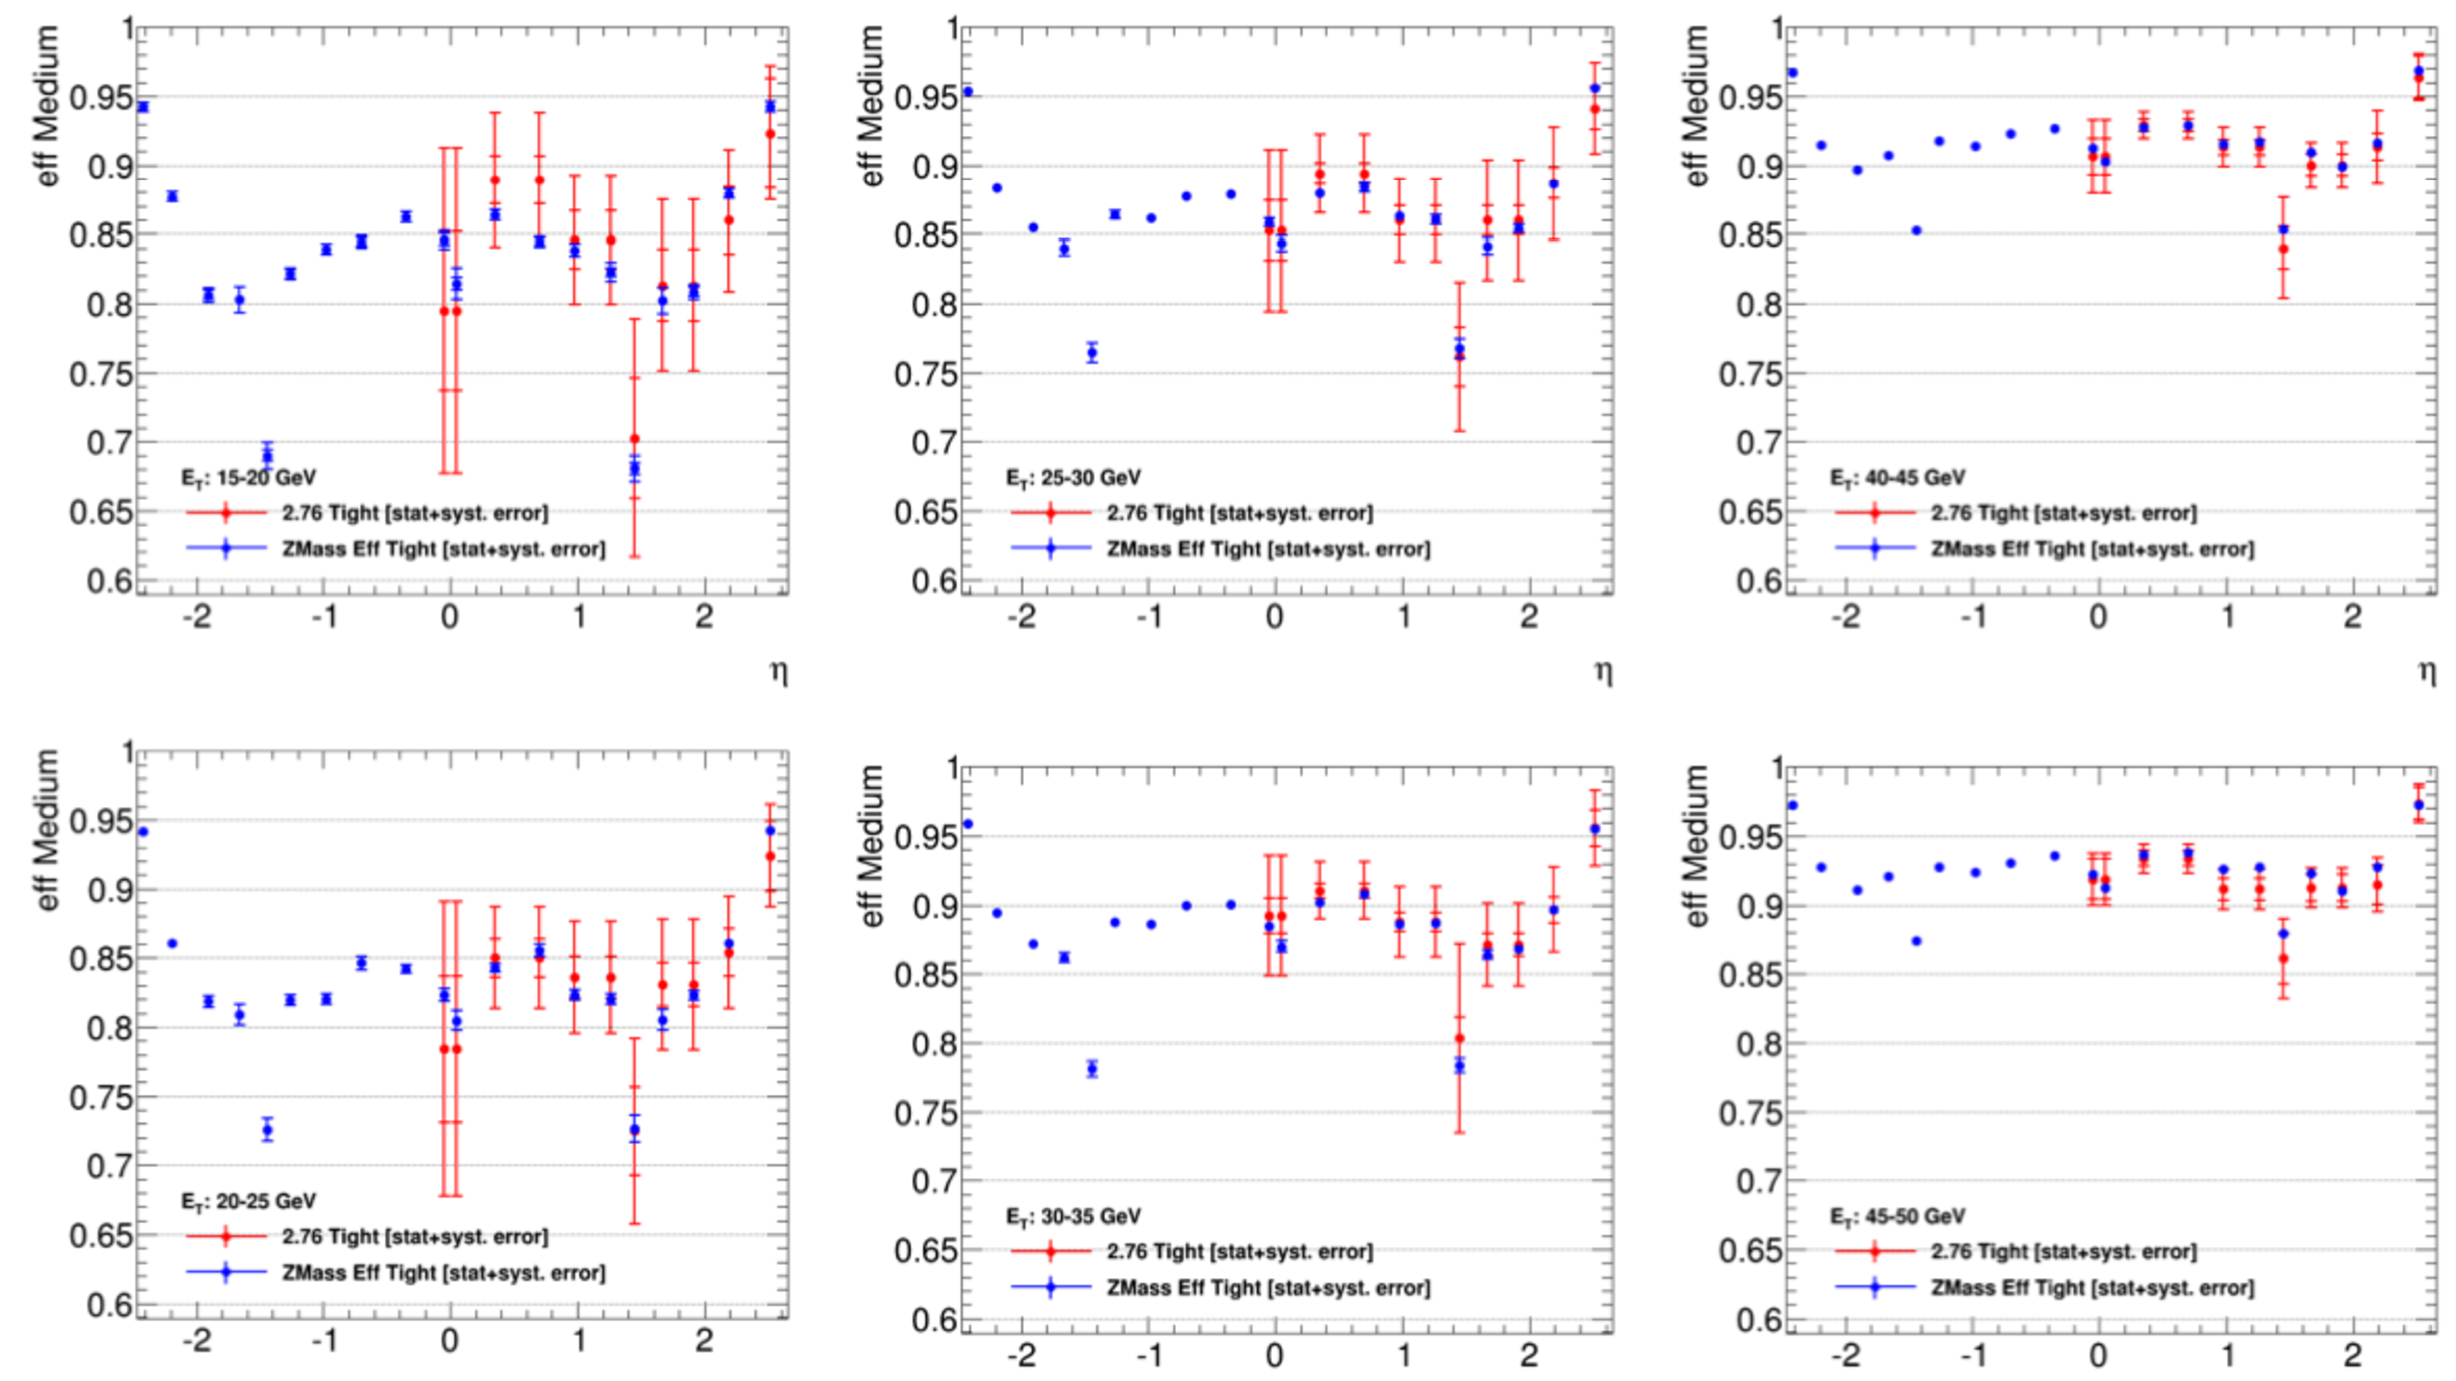
\includegraphics[width=1\textwidth]{MCCorrections/sf.pdf}
\caption{Comparison of electron efficiencies as calculated for 8 TeV (blue points) and 2.76 TeV (red points) for MC simulation. Efficiencies are shown as a function of pseudorapidity ($\eta$) for different electron $E_T$ bins. Both statistical and systematic uncertainties are shown\cite{ElecEff}. }
\label{eff_comp}
\end{figure}

Efficiency in MC simulation is corrected to match lepton efficiencies in data by introducing the relevant scale factor :
\begin{equation}
SF=\frac{\epsilon^{data}}{\epsilon^{MC}},
\end{equation}
where $\epsilon^{data}$ and $\epsilon^{MC}$ are the lepton efficiencies in the data and MC respectively.

Scale factors are calculated  as a function of \ptl and $\eta^{l}$ and have associated statistical and systematic uncertainty components. The statistical component is connected to a size of $Z\to ll$ sample, which in our case is around 500 events per each lepton flavor. This makes the statistical error the dominant one and means that precise calculation of scaling factors based on this data is difficult.

It is possible, however, to use scale factors derived using 8 TeV 2012 data\cite{ElecEff}. The main difference between 2.76 TeV and 8 TeV data samples are center-of-mass energy and the pile-up conditions. The effects of these differences have been studied by the electron performance group at \atlas using $Z\to ee$ MC sample. Fig.~\ref{eff_comp} shows the electron efficiencies for different $E^e$ ranges as a function of $\eta^{e}$, for the MC simulation for $\sqrt{s}$ = 2.76TeV and $\sqrt{s}$ = 8 TeV. The obtained scale factors agree with each other within the uncertainty. This justifies the usage of at 8 TeV scaling factors with increased uncertainty (that is considered to be fully statistical) in the analysis at $\sqrt{s}$ = 2.76 TeV. 

The muon trigger scale factors have to be derived from the $\sqrt{s}$ = 2.76 TeV data since the muon trigger used in the analysis has not been present in the 2012 data. The available statistics of the Z-boson candidates in data does not allow to measure the scale factors as a function of \ptl and $\eta^{l}$.  The selection criteria on muon momentum are significantly higher than a trigger threshold, therefore the $P_T$ dependence of the trigger scale factors can be neglected. Binning in $\eta$ is motivated by the detector construction: $|\eta|<1.05$ corresponds to a barrel part of the muon spectrometer, while $1.05<|\eta|<2.5$ is an end-cap MS (see Sec.~\ref{sec:MuonSys}). The bend of the muon trajectory in the magnetic field can cause differences in a trigger efficiencies for opposite muon charges. Additionally, a possible charge dependency of the scale factors are studied. 

The obtained scale factors with neglected $\eta$ dependency are shown in Tab.~\ref{tab:MuonSF}. The obtained scale factors for different muon charges are not in agreement with each other within the uncertainty, that can be interpreted as a non-negligible charge dependency. The comparison of trigger efficiencies for data and MC simulation as a function of $\eta$ is shown in Fig.~\ref{fig:MuSF}. 

Effect of applying different scale factors on muons for W analysis is shown in Fig.~\ref{fig:SFBined1}-~\ref{fig:SFBined3}. Good agreement between the data and simulation is achieved by applying a non $\eta$-dependent charge-dependent scale factors. Therefore, for this analysis, the $\eta$ dependency of the trigger scale factors is considered to be negligible.

\begin{table}[!t]
    \caption{Overall muon trigger scale factors and their statistical uncertainty.}
	\label{tab:MuonSF}
	\begin{center}
		\begin{tabular}{|l | c | c|}
		\hline
		& SF & SF stat.error\\
		\hline
		\hline
		$\mu$ & 0.988 & 0.011\\
		\hline
		$\mu^{+}$ & 1.012 & 0.015\\
		$\mu^{-}$ & 0.964 & 0.015\\
		\hline
		\end{tabular}
		\end{center}
\end{table}

\begin{figure}[!b]
\minipage{0.32\textwidth}
  \center{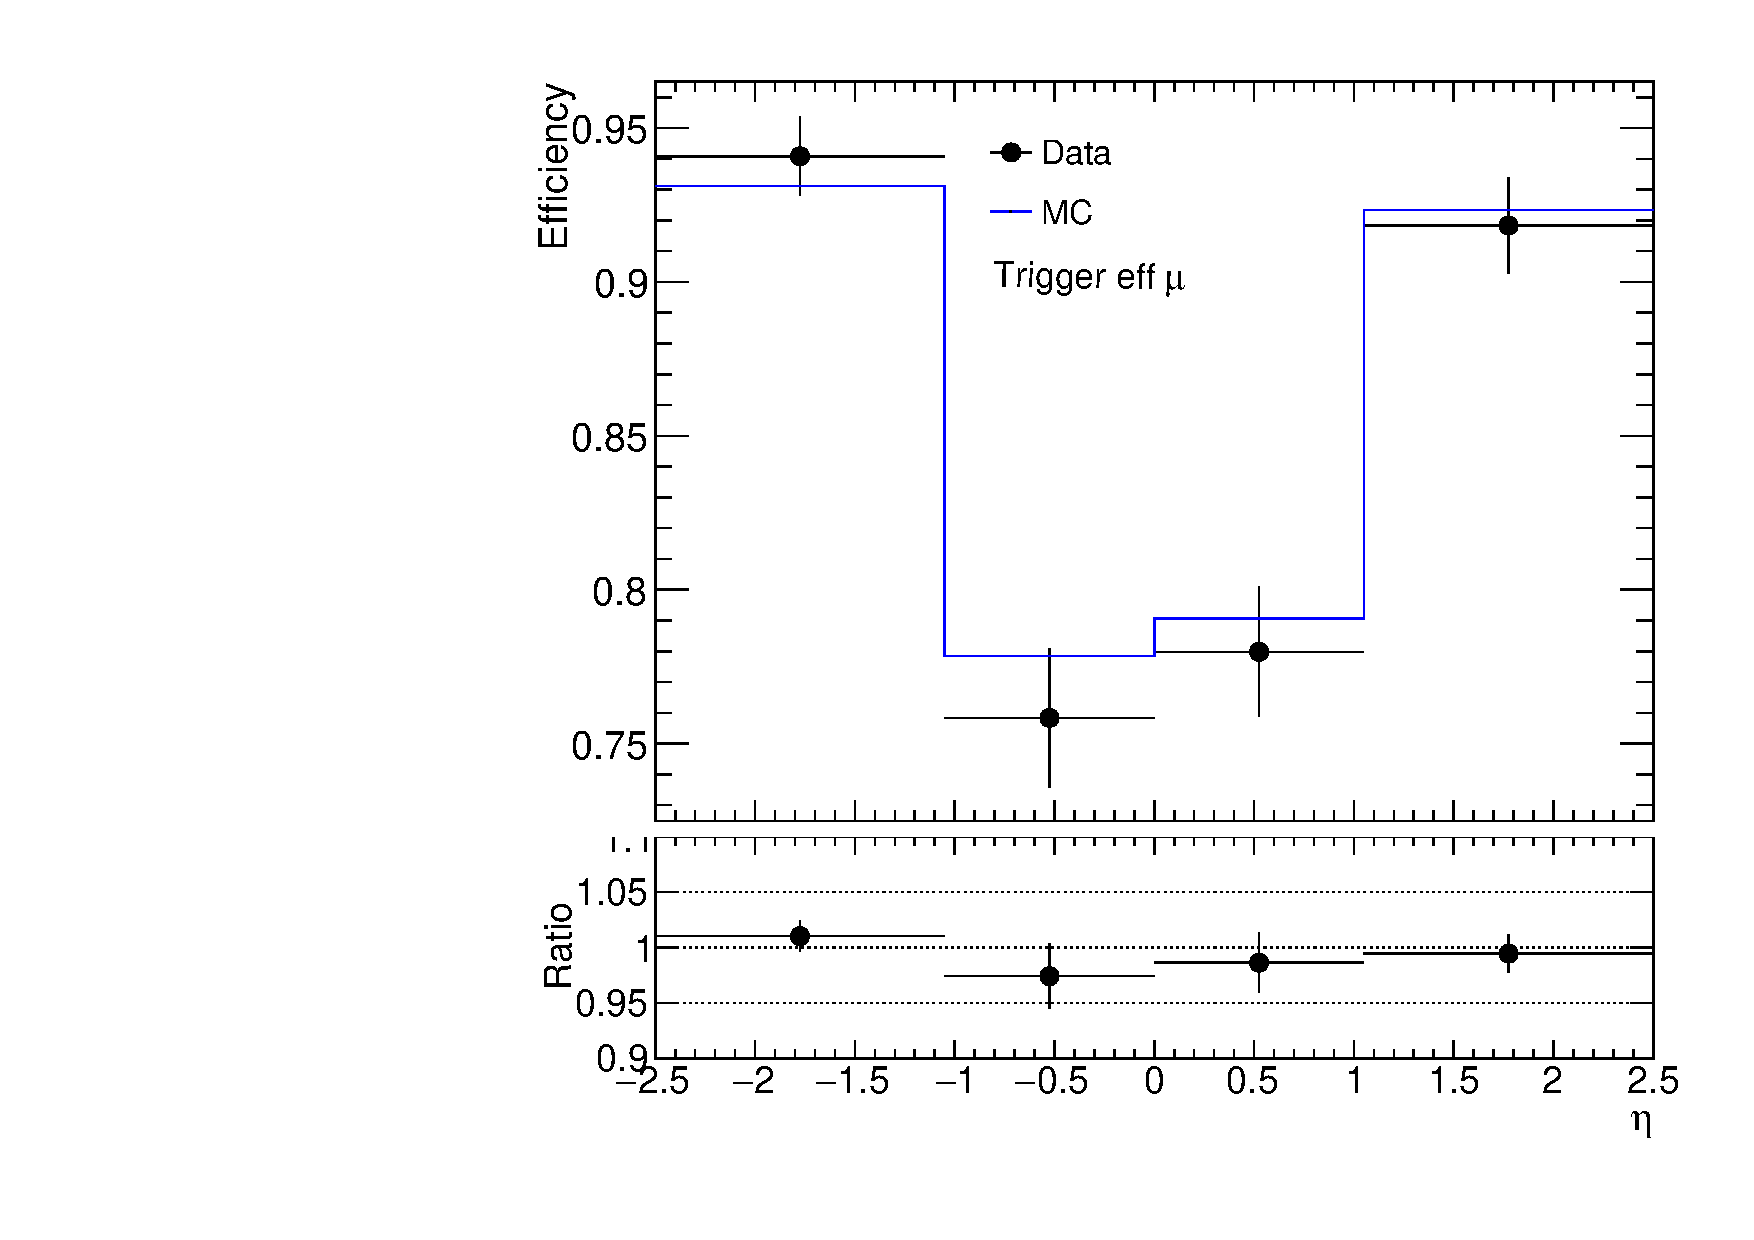
\includegraphics[width=\linewidth]{MCCorrections/m.pdf} \\ a)}
\endminipage\hfill
\minipage{0.32\textwidth}
   \center{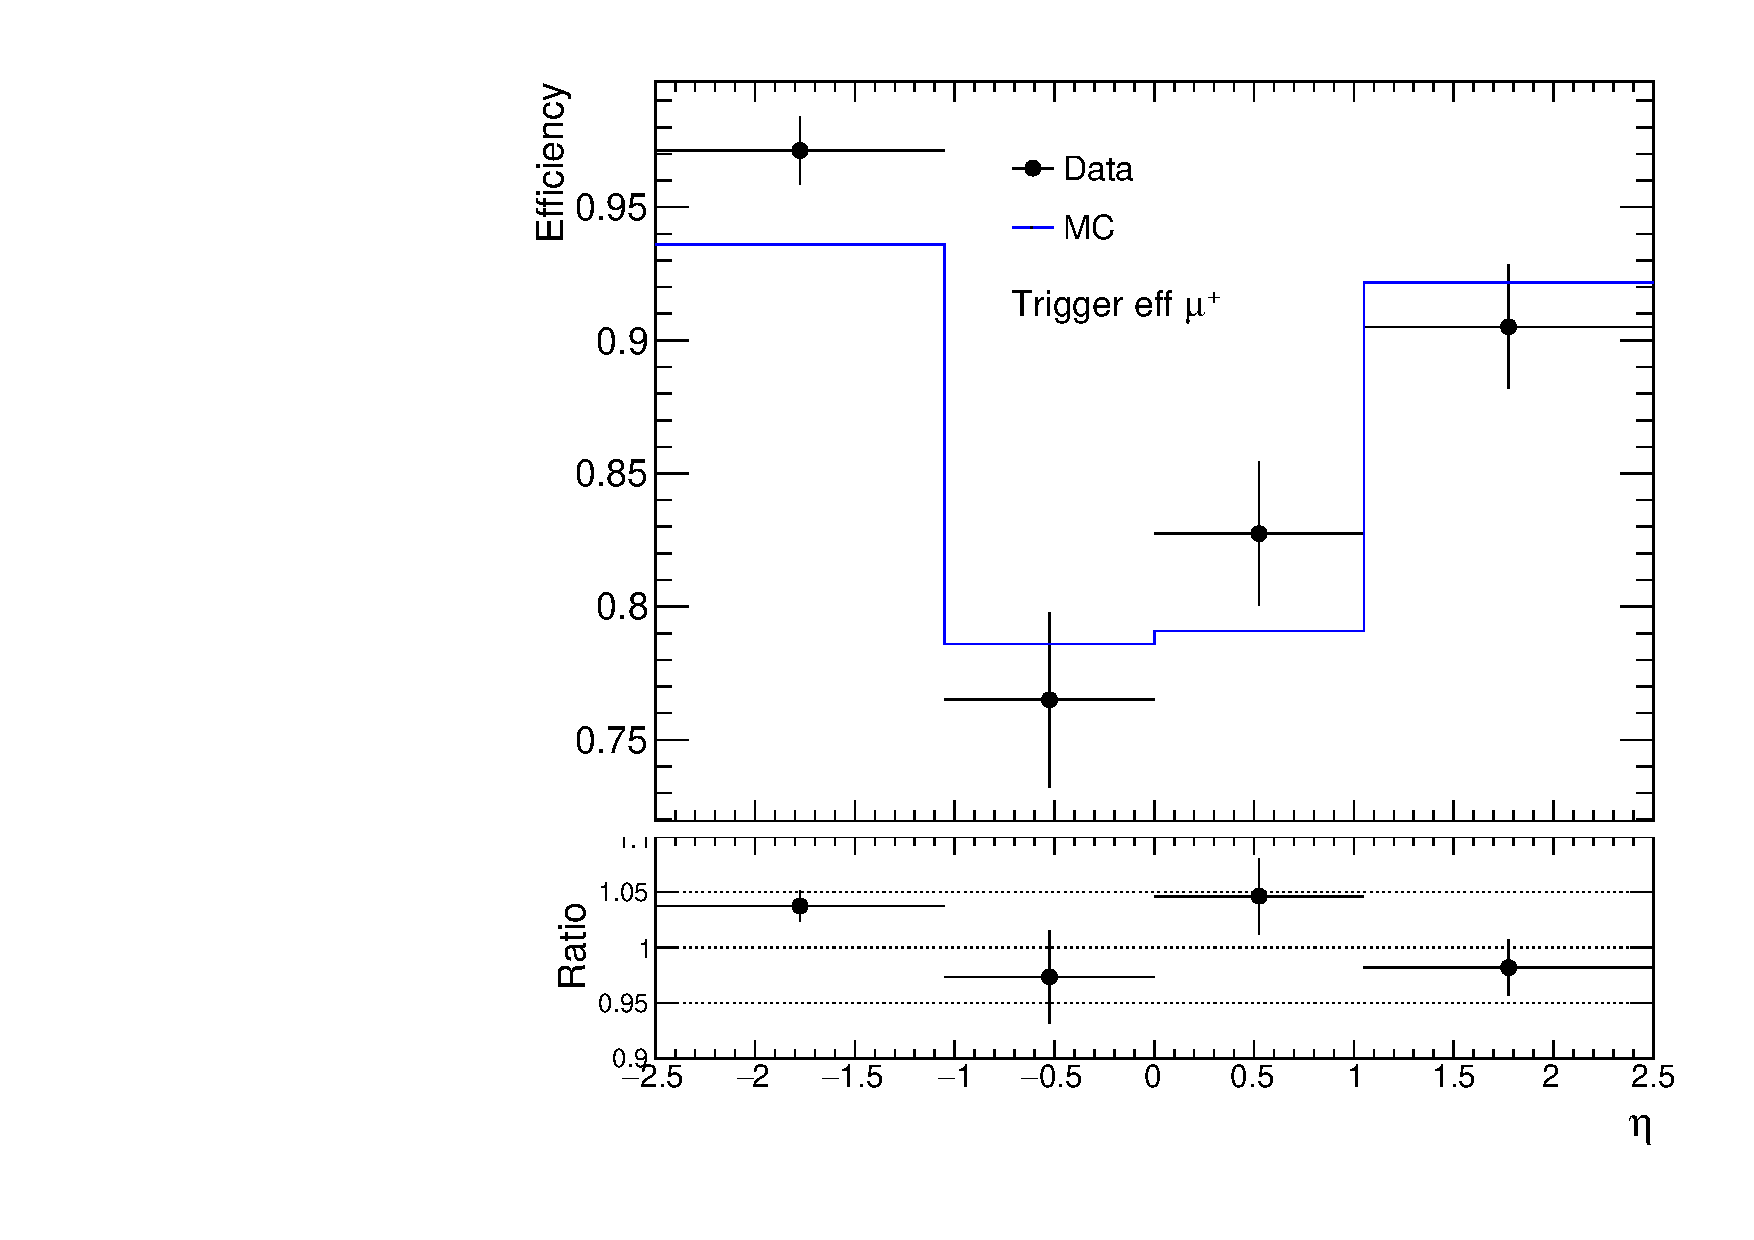
\includegraphics[width=\linewidth]{MCCorrections/mP.pdf} \\ b)}
\endminipage\hfill
\minipage{0.32\textwidth}%
   \center{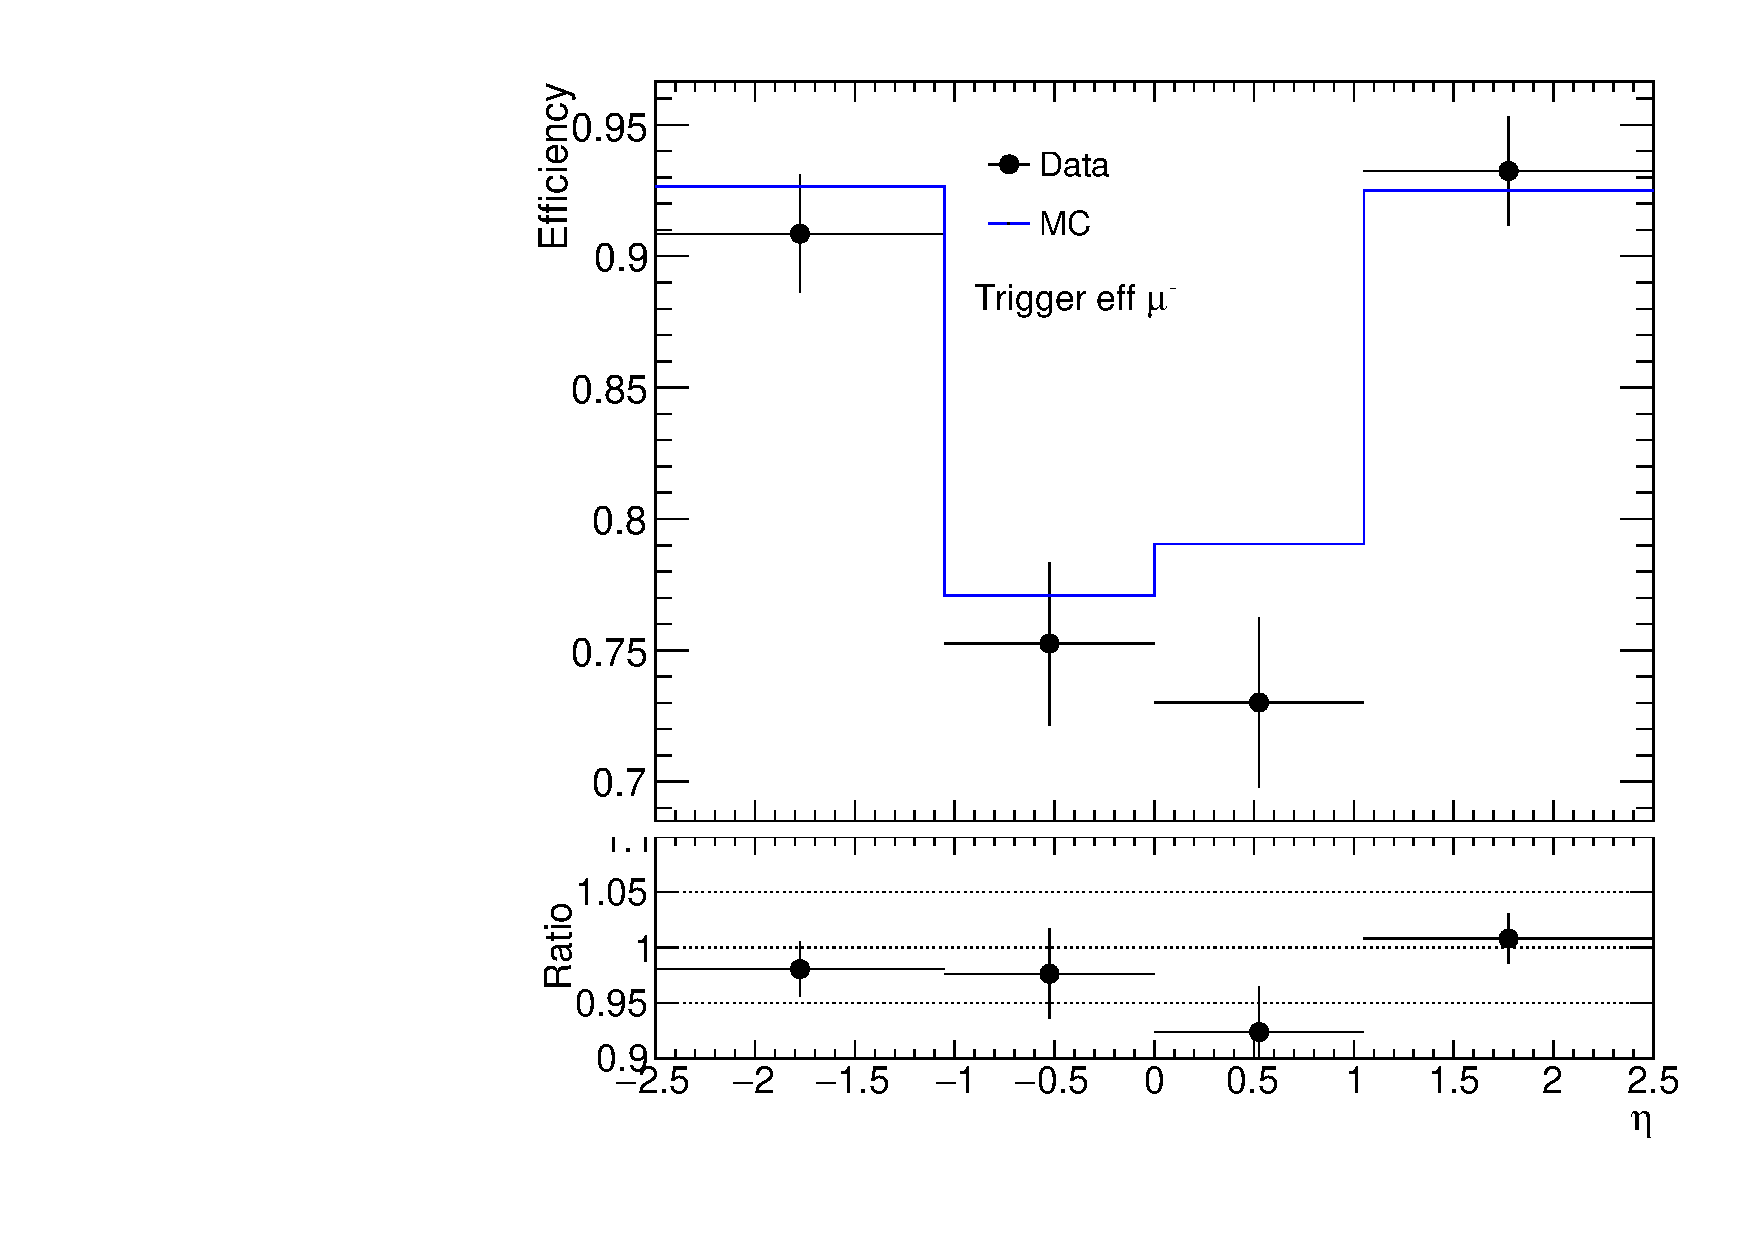
\includegraphics[width=\linewidth]{MCCorrections/mM.pdf} \\ c)}
\endminipage
\caption{Trigger efficiencies for a) $\mu$ b) $\mu^{+}$  c) $\mu^{-}$ as a function of muon pseudorapidity.}
\label{fig:MuSF}
\end{figure}

\begin{figure}[!tbp]
\minipage{0.5\textwidth}
  \center{\includegraphics[width=\linewidth]{MCCorrections/BinnedCharged/Wmu_Boson_lepEtaFine.pdf} \\ a)}
\endminipage\hfill
\minipage{0.5\textwidth}
  \center{\includegraphics[width=\linewidth]{MCCorrections/OneBinCharged/Wmu_Boson_lepEtaFine.pdf} \\ b)}
\endminipage\hfill
\caption{Muon pseudorapidity distribution for the $W\to \mu \nu$  event selection with a) binned  b) not binned charge dependent trigger scale factor applied.}
\label{fig:SFBined1}
\end{figure}

\begin{figure}[!tbp]
\minipage{0.5\textwidth}
  \center{\includegraphics[width=\linewidth]{MCCorrections/BinnedCharged/Wmu_Plus_lepEtaFine.pdf} \\ a)}
\endminipage\hfill
\minipage{0.5\textwidth}
  \center{\includegraphics[width=\linewidth]{MCCorrections/OneBinCharged/Wmu_Plus_lepEtaFine.pdf} \\ b)}
\endminipage\hfill
\caption{Muon pseudorapidity distribution for the $W\to \mu^{+} \nu$  event selection with  a) binned  b) not binned charge dependent trigger scale factor applied.}
\label{fig:SFBined2}
\end{figure}

\begin{figure}[!tbp]
\minipage{0.5\textwidth}
  \center{\includegraphics[width=\linewidth]{MCCorrections/BinnedCharged/Wmu_Minus_lepEtaFine.pdf} \\ a)}
\endminipage\hfill
\minipage{0.5\textwidth}
  \center{\includegraphics[width=\linewidth]{MCCorrections/OneBinCharged/Wmu_Minus_lepEtaFine.pdf} \\ b)}
\endminipage\hfill
\caption{Muon pseudorapidity distribution for the $W\to \mu^{-} \nu$  event selection with a) binned  b) not binned charge dependent trigger scale factor applied.}
\label{fig:SFBined3}
\end{figure}

\section{Electron energy scale and resolution correction}\label{sec:elecScale}
The possible shift in the reconstructed energy of the electron is corrected as a three step procedure\cite{ElecCalib}:
\begin{itemize}
\item Calibration of electronics, which matches a raw signal from readout electronics to a cluster energy deposit.
\item MC based $e/\gamma$ response calibration, that corrects effects of the energy loss in the material in front of the calorimeter and the leakage into the hadronic calorimeter. This calibration is applied on both data and MC.
\item Correction of the calorimeter cell response in the data, which corrects the  response variations in specific detector regions.
\end{itemize}

The overall energy shift is parameterized, as:
\begin{equation}
E^{data}=E^{MC}(1+\alpha),
\end{equation}
where $E^{data}$ and $E^{MC}$ are the energies in data and simulation, respectively and $\alpha$ is a mean shift. The effect of this miscalibration on a reconstructed mass of the Z boson, neglecting second order terms is:
\begin{equation}
M^{data}=M^{MC}(1+\alpha), \quad \alpha_{1,2} \sim \frac{\alpha_1+\alpha_2}{2}, 
\end{equation}
where $M{data}$ and $M{MC}$ are the reconstructed mass of the Z-boson for data and MC simulation respectively and $\alpha_i$ is the mean energy shift of the $i$-th electron from the Z-boson decay. 

Additionally, the difference between data and MC simulation in the electron energy resolution is taken into account. The general dependency of electron energy resolution on its energy is described by Eq.~\ref{eq:EMResoultion}. It is assumed, that the sampling and the noise terms are well modeled by the MC simulation and the main difference comes from a constant term. 
So, the electron energy resolution correction can be written as:
\begin{equation}
\frac{\sigma_E}{E}^{Data}=\frac{\sigma_E}{E}^{MC} \oplus c,
\end{equation}
where $c$ is a resolution correction. Similarly to the electron energy scale correction, it is possible to derive electron energy resolution correction factor by comparing $M^{data}$ and $M^{MC}$ distributions. 

The values $\alpha$ and $c$ are obtained using the $\chi^2$-based fit of an invariant mass of electron pairs in data and MC. 

\section{Muon momentum correction}\label{sec:MuonMomCor}
Muon momentum resolution depends on $\eta$, $\phi$ and $P_T$ of the muon \cite{AtlasExperiment}. There is an empirical formula to describe this dependence in the detector (ID or MS)\cite{MuonCalib}:
\begin{equation}\label{eq:MuonResolution}
\frac{\sigma_{Det}(P_T)}{P_T}=\frac{r^{Det}_0(\eta, \phi)}{P_T} \oplus r^{Det}_1 (\eta, \phi)  \oplus r^{Det}_2(\eta, \phi) \cdot P_T.
\end{equation}
The first term ($\frac{r^{Det}_0(\eta, \phi)}{P_T}$) originates from the fluctuations of the energy loss in the material. The second term ( $r^{Det}_1$ ) comes  from the magnetic field non-homogeneities. The third term ($r^{Det}_2$) describes the intrinsic resolution effects. 

Similarly to electrons, the overall muon momentum scale shift between data and MC is parameterized as:
\begin{equation}
P_T^{data}=P_T^{MC}+s_0^{Det}(\eta, \phi)+s_1^{Det}(\eta, \phi) \cdot P_T^{MC},
\end{equation}
where $s_0^{Det}(\eta, \phi)$ comes from the imperfect knowledge of energy losses for muons passing through the detector. 

This leads to an overall correction formula:
\begin{equation}
P^{Cor,Det}_T=\frac{P_{T}^{MC,Det}+\sum\limits_{n=0}^1 s_n^{Det}(\eta, \phi)(P_T^{MC,Det})^n}{1+\sum\limits_{m=0}^2 \Delta r_m^{Det}(\eta, \phi)(P_T^{MC,Det})^{m-1} g_m},
\end{equation}
where $g_m$ are normally distributed random variables (with the mean 0 and the standard deviation 1). Due to a small amount of material in the ID, $\Delta r^{ID}_0(\eta, \phi)$ and $s_0^{ID}(\eta, \phi)$ are set to 0. The misalignment effect of the MS is corrected in simulation by adding a random smearing to the  MS alignment constants. This allows to set $\Delta r^{MS}_2(\eta, \phi)$ = 0 during the fit procedure. 

The relevant correction factors are extracted using events from $Z \to \mu \mu$ decays, where both muon candidates fulfill the combined muon criteria described in Sec.\ref{sec:MuonRec}. The correction extraction is performed first for the ID part and then for the MS part using the distribution of the mass of the lepton pair reconstructed in ID and MS. Additionally, the following fit variable is considered:
\begin{equation}
\rho = \frac{P_T^{MS}-P_T^{ID}}{P_T^{ID}},
\end{equation}
which represents the $P_T$ imbalance (the difference between the ID and the MS). 

The momentum correction factors are propagated to the combined muon momentum, using a weighted average:
\begin{equation}
P_T^{Cor,CB}= f\cdot P_T^{Cor,ID}+(1-f) \cdot P_T^{Cor,MS},
\end{equation}
where the weight $f$ is measured in MC simulation using the same equation. 
